	% TeX шаблон, пример оформления отчёта по лабораторной работе.
% Автор: Шмаков И.А.
% Версия от: 05 ноября 2018 года.
% Сборка документа из командной строки:
% ~$ pdflatex -shell-escape main.tex

\documentclass[a4paper,14pt]{extarticle}
\usepackage[utf8]{inputenc}
\usepackage[T2A]{fontenc}
\usepackage[english,russian]{babel}

% одинарный интервал
\usepackage{setspace}
\singlespacing 

\usepackage[left=3cm, right=1cm, top=1.5cm, bottom=1.5cm]{geometry}
\usepackage{icomma} % "Умная" запятая: $0,2$ --- число, $0, 2$ --- перечисление
\usepackage{indentfirst} % Красная строка.

% для гиперссылок и выделение их цветом
\usepackage{xcolor}
\usepackage{hyperref}

 % Цвета для гиперссылок
\definecolor{linkcolor}{HTML}{000000} % цвет ссылок
\definecolor{urlcolor}{HTML}{799B03} % цвет гиперссылок
\hypersetup{pdfstartview=FitH,  linkcolor=linkcolor, urlcolor=urlcolor, colorlinks=true}

% Пакет отвечающий за листинги.
\usepackage[outputdir=build]{minted} 
\renewcommand\listingscaption{Листин}
% Фикс "red box" в minted 
\usemintedstyle{xcode}

% Подключение графики
\usepackage{graphicx}
\usepackage{float}

\usepackage{amsmath}

\renewcommand{\thesection}{\arabic{section}}

\begin{document}
\begin{titlepage}
  \begin{center}
    \MakeUppercase{Министерство науки и высшего образования Российской Федерации} \\
    \MakeUppercase{ФГБОУ ВО Алтайский государственный университет}
    \vspace{0.25cm}
    
    Физико-технический факультет
    
    Кафедра вычислительной техники и электроники
    \vfill
    
    \textsc{Отчёт по лабораторной работе №1 по курсу \\ <<Практикум по ТРПО>>}
  \bigskip

\end{center}
\vfill

\newlength{\ML}
\settowidth{\ML}{«\underline{\hspace{0.6cm}}» \underline{\hspace{2cm}}}
\hfill\begin{minipage}{0.5\textwidth}
  Выполнил студент 4-го курса, \\ 576 группы:\\
  \underline{\hspace{\ML}} В.\,Е.~Щербаков\\
  «\underline{\hspace{0.7cm}}» \underline{\hspace{2cm}} \the\year~г.
\end{minipage}%
\bigskip

\settowidth{\ML}{«\underline{\hspace{0.6cm}}» \underline{\hspace{2cm}}}
\hfill\begin{minipage}{0.5\textwidth}
  Проверил\\
  \underline{\hspace{\ML}} П.\,Н.~Уланов\\
  «\underline{\hspace{0.7cm}}» \underline{\hspace{2cm}} \the\year~г.
\end{minipage}%
\vfill

\begin{center}
  Барнаул, \the\year~г.
\end{center}
\end{titlepage}

\tableofcontents

\newpage

\section{Введение и постановка задачи}
Изучение принципов параллельного программирования на примере потенциально высокопараллельного алгоритма нахождения числа $\pi$.

\section{Теоретическое описание задачи}
У нас есть квадрат со стороной длиной r и вписанная в него четверть окружности с радиусом r. Необходимо случайным образом «кидать» точки в квадрат. Если точка попадает в область окружности, то увеличиваем счетчик попаданий на единицу.

\begin{align*}
S_{okr} = \frac{\pi r^2}{4}
\end{align*}

Площадь квадрата:
\begin{align*}
S_{kvad} = r^2
\end{align*}

Отношение площадей:
\begin{align*}
\frac{S_{okr}}{S_{kvad}} = \frac{\pi r^2}{4r^2} = \frac{\pi}{4}
\end{align*}

\newpage

\section{Алгоритм и блок-схема}			
Блок-схема программы:	
\begin{figure}[H]
	\centering
	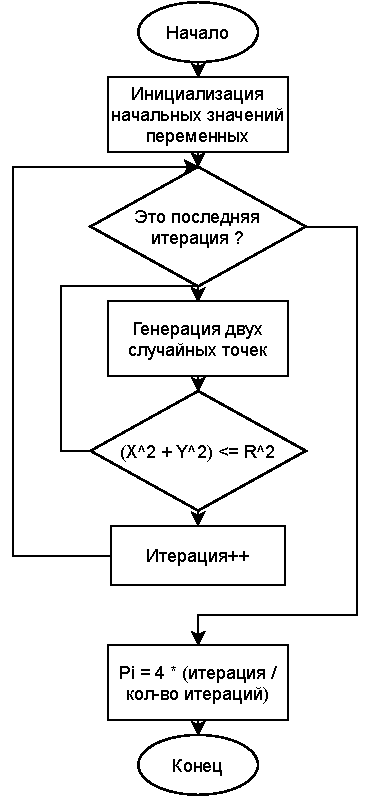
\includegraphics[page=1, width=0.6\textwidth]{include/block_scheme.pdf}
	\caption{Блок-схема программы}
\end{figure}

\newpage

\section{Проверка работы программы}
Для проверки работы программы напишем простой Makefile, дабы облегчить себе задачу, его код приведен ниже в приложении \ref{makefile}

Все нижеприведенные вычисления были произведены на процессоре Ryzen 3700x@4.2 GHz, при использовании OpenMPI были задействованы все 16 потоков.

\begin{minted}{bash}
g++ -O3 -march=native serial.cpp -o lab3_serial
g++ -O3 -march=native -fopenmp parallel.cpp -o lab3_parallel
Benching serial code...
Примерно равно: 3.14251

real    0m16,557s
user    0m16,552s
sys     0m0,000s
Benching parallel code...
Примерно равно: 3.13259

real    0m19,063s
user    4m36,851s
sys     0m0,000s
\end{minted}

Как мы видим, распараллеливание алгоритма через OpenMPI не дало должного прироста производительности.

\addcontentsline{toc}{section}{Приложение}
\section*{Приложение}

\subsection*{Листинг serial.cpp}
\addcontentsline{toc}{subsubsection}{Листинг serial.cpp}
\inputminted[mathescape,linenos,breaklines]{c++}{../src/serial.cpp}

\subsection*{Листинг parallel.cpp}
\addcontentsline{toc}{subsubsection}{Листинг parallel.cpp}
\inputminted[mathescape,linenos,breaklines]{c++}{../src/parallel.cpp}

\subsection*{Листинг Makefile}
\label{makefile}
\addcontentsline{toc}{subsubsection}{Листинг Makefile}
\inputminted[mathescape,linenos,breaklines]{make}{../src/Makefile}
\end{document}          
